\documentclass[aspectratio=169]{beamer}

% Theme Selection
\usetheme{Madrid}
\usecolortheme{beaver}

% Packages
\usepackage{amsmath}
\usepackage{amssymb}
\usepackage{algorithm}
\usepackage{algpseudocode}
\usepackage{graphicx}
\usepackage{tikz}
\usepackage{booktabs} % For nicer tables
\usepackage{multimedia}

% Title Information
\title[Advanced Analysis of 1DBPP]{A Comparative Analysis of Approximation Algorithms for the One-Dimensional Bin Packing Problem}
\subtitle{From Greedy Heuristics to Discrepancy Theory}
\author[Team Alan Turing]{
    \textbf{Team Alan Turing} \\
    Aman Jayesh, Mukund Hebbar, \\
    Pranav Swarup Kumar, \\
    Shreyas Ramasubramanian, Shreyash Chandak
}
\date{\today}

\begin{document}

% -----------------------------------------------------------------------------
% INTRODUCTION
% -----------------------------------------------------------------------------

\begin{frame}
    \titlepage
\end{frame}

\begin{frame}{Table of Contents}
    \tableofcontents
\end{frame}

\section{Introduction \& Complexity}

\begin{frame}{Problem Definition \& Hardness}
    \begin{block}{The 1D Bin Packing Problem (1DBPP)}
        Given items $I = \{s_1, ..., s_n\}$ with $s_i \in (0, 1]$, pack them into minimum $m$ unit-capacity bins.
    \end{block}

    \textbf{The Inapproximability Barrier:}
    \begin{itemize}
        \item By reduction from \textsc{Partition}, distinguishing between $OPT=2$ and $OPT=3$ is NP-Hard.
        \item \textbf{Theorem:} No polynomial-time algorithm can achieve an approximation ratio better than $3/2$ unless P=NP.
        \item \textbf{Implication:} We must settle for:
        \begin{enumerate}
            \item Asymptotic Guarantees ($OPT \to \infty$).
            \item Schemes dependent on $\epsilon$ (APTAS).
            \item Additive Error terms (e.g., $OPT + C$).
        \end{enumerate}
    \end{itemize}
\end{frame}

% -----------------------------------------------------------------------------
% FOUNDATIONAL HEURISTICS
% -----------------------------------------------------------------------------

\section{Foundational Heuristics}

\begin{frame}{Online Heuristic 1: First-Fit (FF)}
    \textbf{Mechanics:}
    \begin{itemize}
        \item Process items in order of arrival $s_1, s_2, \dots, s_n$.
        \item Place item $s_i$ in the \textbf{first} bin $B_j$ ($j=1 \dots k$) where it fits.
        \item If it fits nowhere, open a new bin $B_{k+1}$.
    \end{itemize}

    \textbf{Complexity:}
    \begin{itemize}
        \item Naive: $O(n^2)$.
        \item Optimized: $O(n \log n)$ using Segment Trees to query the first valid bin.
    \end{itemize}

    \begin{block}{Theoretical Bound (Theorem 1)}
        $$ FF(L) \le 1.7 \cdot OPT(L) + 2 $$
        \textit{Note:} FF tends to leave larger, contiguous gaps in earlier bins, which helps accommodate future items.
    \end{block}
\end{frame}

\begin{frame}{Online Heuristic 2: Best-Fit (BF)}
    \textbf{Mechanics:}
    \begin{itemize}
        \item Place item $s_i$ in the bin with the \textbf{minimum residual capacity} sufficient to hold it.
        \item Goal: ``Tightest fit'' to minimize immediate waste.
    \end{itemize}

    \textbf{The ``Sand'' Problem (Fragmentation):}
    \begin{itemize}
        \item BF creates bins that are nearly full but contain tiny, unusable gaps (``sand'').
        \item These splinters are often too small for any future item, rendering that capacity wasted.
    \end{itemize}

    \begin{block}{Theoretical Bound (Theorem 2)}
        $$ BF(L) \le 1.7 \cdot OPT(L) + C $$
        Despite the strategy difference, it shares the same worst-case ratio as FF.
    \end{block}
\end{frame}

\begin{frame}{Offline Heuristics: FFD \& BFD}
    \textbf{The Power of Pre-processing:}
    \begin{itemize}
        \item \textbf{Rule:} Sort items such that $s_1 \ge s_2 \ge \dots \ge s_n$.
        \item \textbf{Intuition:} Placing ``big rocks'' first ensures difficult items are packed when bins have maximum capacity. Small items (``sand'') fill the remaining gaps later.
    \end{itemize}

    \textbf{Algorithms:}
    \begin{itemize}
        \item \textbf{First-Fit Decreasing (FFD):} Sort, then run First-Fit.
        \item \textbf{Best-Fit Decreasing (BFD):} Sort, then run Best-Fit.
    \end{itemize}

    \begin{alertblock}{Johnson's Theorem \& Dósa's Tight Bound (2007)}
        Sorting improves the approximation ratio significantly:
        $$ FFD(L) \le \frac{11}{9} OPT(L) + \frac{6}{9} \approx 1.22 \cdot OPT(L) $$
    \end{alertblock}
\end{frame}

\begin{frame}{Qualitative Comparison: FF vs. BF}
    Although they have the same worst-case bound (1.7), their average-case behavior differs due to \textbf{Space Fragmentation}.
    
    \begin{table}[]
        \centering
        \begin{tabular}{p{5cm} p{5cm}}
        \toprule
        \textbf{First-Fit Strategy} & \textbf{Best-Fit Strategy} \\
        \midrule
        Oblivious to ``tightness''. & Minimizes local residual space. \\
        \midrule
        Leaves \textbf{large, contiguous gaps} in early bins. & Creates many \textbf{tiny, unusable gaps} (``sand''). \\
        \midrule
        Statistically better for accommodating future medium-sized items. & Risk of ``suffocating'' on future items slightly larger than the gaps. \\
        \bottomrule
        \end{tabular}
    \end{table}
\end{frame}

\begin{frame}{Advanced Online: Harmonic-k Algorithm}
    \textbf{Concept:} Unlike FF/BF, Harmonic-$k$ classifies items by size intervals to limit fragmentation.
    
    \begin{block}{Mechanism}
        \begin{enumerate}
            \item Divide the interval $(0, 1]$ into $k$ sub-intervals: 
            $$ I_j = (\frac{1}{j+1}, \frac{1}{j}] \text{ for } j=1 \dots k-1, \text{ and } I_k = (0, \frac{1}{k}] $$
            \item \textbf{Dedicated Bins:} Items of type $I_j$ are \textbf{only} packed into bins dedicated to type $j$.
            \item \textbf{Packing Rule:} A bin for type $j$ can hold exactly $j$ items (since $s_i > \frac{1}{j+1}$ implies $j+1$ items would exceed capacity, but $s_i \le \frac{1}{j}$ allows $j$ items).
        \end{enumerate}
    \end{block}

    \textbf{Performance:}
    \begin{itemize}
        \item As $k \to \infty$, the asymptotic approximation ratio improves.
        \item \textbf{Limit:} $\Pi_\infty \approx 1.6910$ (Better than FF/BF's 1.7).
        \item \textbf{Trade-off:} Reduces flexibility but guarantees bounded space wastage per bin type.
    \end{itemize}
\end{frame}

% -----------------------------------------------------------------------------
% APTAS (Fernandez de la Vega & Lueker)
% -----------------------------------------------------------------------------

\section{APTAS Framework}

\begin{frame}{Phase 2: APTAS (Fernandez de la Vega \& Lueker)}
    \textbf{Goal:} Achieve $(1+\epsilon)OPT + O(1)$ for any fixed $\epsilon > 0$.
    
    \begin{alertblock}{The 4-Step Framework}
    \begin{enumerate}
        \item \textbf{Eliminate Small Items:} Temporarily discard items $< \epsilon/2$.
        \item \textbf{Linear Grouping:} Round sizes to reduce instance complexity.
        \item \textbf{Exact Solution:} Solve the restricted instance using DP/IP.
        \item \textbf{Reinsertion:} Add small items back into gaps.
    \end{enumerate}
    \end{alertblock}
\end{frame}

\begin{frame}{APTAS Step 2: Linear Grouping (The Core Mechanic)}
    To solve the problem exactly, we must reduce the number of distinct item sizes to a constant $K$.
    
    \textbf{Procedure:}
    \begin{enumerate}
        \item Sort large items in descending order.
        \item Partition them into $1/\epsilon^2$ groups of size $k$ (where $k \approx \epsilon \cdot OPT$).
        \item \textbf{Rounding:} In each group, round all items \textit{up} to the size of the largest item in that group.
    \end{enumerate}
    
    \begin{block}{Proof Sketch (Grouping Error)}
        Let $L$ be the original list and $L'$ be the rounded list.
        Because we round up, $L'$ dominates $L$.
        However, the rounded items of group $i$ are equal to the smallest items of group $i-1$.
        Thus, we can essentially ``shift'' the packing.
        $$ OPT(L') \le OPT(L) + k \text{ (items)} \approx (1+\epsilon)OPT $$
    \end{block}
\end{frame}

\begin{frame}{APTAS Steps 3 \& 4: Solving and Unrounding}
    \textbf{Step 3: Solve Bounded Instance}
    \begin{itemize}
        \item With constant distinct sizes, the number of valid bin \textit{configurations} is constant.
        \item We solve this using Integer Programming (IP) in constant dimensions ($O(1)$ variables), which takes constant time for fixed $\epsilon$.
    \end{itemize}

    \textbf{Step 4: Unrounding \& Reinsertion}
    \begin{itemize}
        \item Replace rounded items with original sizes (valid because $size(orig) \le size(rounded)$).
        \item Grease the small items ($< \epsilon/2$) into remaining gaps using First-Fit.
        \item If a small item doesn't fit, open a new bin. Since items are small, these extra bins are densely packed, incurring negligible cost.
    \end{itemize}
    
    \textbf{Result:} $A_{\epsilon}(I) \le (1+\epsilon)OPT + 1$.
\end{frame}

% -----------------------------------------------------------------------------
% KARMARKAR-KARP (1982)
% -----------------------------------------------------------------------------

\section{Karmarkar-Karp (1982)}

\begin{frame}{The Additive Breakthrough: Karmarkar-Karp (KK82)}
    For 30 years, this was the theoretical benchmark.
    
    \begin{block}{The Guarantee}
        $$ A(I) \le OPT(I) + O(\log^2 OPT(I)) $$
    \end{block}
    
    This effectively eliminates the multiplicative error ($\epsilon \cdot OPT$) seen in APTAS.
    
    \textbf{Key Innovations:}
    \begin{enumerate}
        \item \textbf{Gilmore-Gomory LP:} Formulating the problem based on Patterns.
        \item \textbf{Ellipsoid Method + Knapsack Oracle:} Solving exponential constraints efficiently.
        \item \textbf{Iterative Rounding:} A loop that solves a sequence of diminishing residual problems.
    \end{enumerate}
\end{frame}

\begin{frame}{Mechanism 1: Solving the Exponential LP}
    The Configuration LP has a variable $x_p$ for every valid pattern $p$ (exponential number of variables).
    
    \textbf{The Dual Solution:}
    \begin{itemize}
        \item We consider the \textit{Dual LP}, which has polynomial variables but exponential constraints.
        \item To solve this using the \textbf{Ellipsoid Method}, we need a \textbf{Separation Oracle}.
        \item The Oracle must find if any constraint is violated, which corresponds to finding the pattern with maximum ``profit'' (dual values).
        \item \textbf{The ``Aha!'' Moment:} Finding the max profit pattern is exactly the \textbf{Knapsack Problem}.
        \item Since Knapsack has an FPTAS, we can solve the LP to near-optimality in polynomial time.
    \end{itemize}
\end{frame}

\begin{frame}{Mechanism 2: Iterative Rounding Procedure}
    We cannot simply round $x_p$ values because standard rounding introduces linear error. KK82 uses a refined loop:
    
    \begin{algorithmic}[1]
        \While{Instance is large}
            \State \textbf{1. Solve LP} to get fractional solution $x$.
            \State \textbf{2. Integral Packing:} Take $\lfloor x_p \rfloor$ bins of each pattern.
            \State \textbf{3. Residual:} Collect the fractional remainders ($x_p - \lfloor x_p \rfloor$) as a new instance $I_{res}$.
            \State \textbf{4. Grouping:} Apply \textit{Geometric Grouping} to $I_{res}$ to reduce item types.
            \State \textbf{5. Repeat} with the reduced residual instance.
        \EndWhile
    \end{algorithmic}
\end{frame}

\begin{frame}{Proof Sketch: The $O(\log^2 OPT)$ Bound}
    Why $\log^2 OPT$?
    
    \begin{enumerate}
        \item \textbf{Geometric Decay:} The size of the residual instance $I_{res}$ drops by a constant factor (e.g., half) in each iteration.
        \item \textbf{Loop Count:} Therefore, the loop runs $T = O(\log n)$ times.
        \item \textbf{Error Accumulation:}
        \begin{itemize}
            \item In each iteration $t$, the Geometric Grouping step introduces a small additive error $E_t$.
            \item This error is bounded: $E_t \approx O(\log (\text{item size constraint}))$.
            \item Summing errors over $O(\log n)$ iterations:
            $$ \sum_{t=1}^{\log n} O(\log n) \approx O(\log^2 n) \approx O(\log^2 OPT) $$
        \end{itemize}
    \end{enumerate}
\end{frame}

% -----------------------------------------------------------------------------
% MODERN BREAKTHROUGHS (Rothvoss)
% -----------------------------------------------------------------------------

\section{Modern Breakthroughs (2013-2015)}

\begin{frame}{Breaking the Barrier: Rothvoß (2013)}
    \textbf{The Problem with KK82:}
    ``Spiky'' patterns (bins with many copies of one small item) caused the $O(\log^2 OPT)$ error during the rounding phase.
    
    \textbf{The 2013 Solution:}
    \begin{itemize}
        \item \textbf{Discrepancy Theory:} Uses the \textit{Lovett-Meka} Constructive Partial Coloring Lemma.
        \item \textbf{Gluing:} Conceptually ``glues'' small items together to smooth out spiky patterns.
        \item \textbf{Result:} Improved bound to $OPT + O(\log OPT \cdot \log \log OPT)$.
    \end{itemize}
\end{frame}

\begin{frame}{Hoberg \& Rothvoß (2015): The Tight Bound}
    To reach the optimal additive gap, they fundamentally restructured the packing process.
    
    \textbf{The 2-Stage Packing Mechanism:}
    \begin{enumerate}
        \item \textbf{Stage 1 (Items $\to$ Containers):} Pack items into ``Containers'' (multisets fitting in a bin).
        \item \textbf{Stage 2 (Containers $\to$ Bins):} Pack Containers into Bins.
    \end{enumerate}
    
    \begin{block}{Why this works?}
        Containers inherently limit the number of copies of any object in a pattern (structural smoothness).
        Applying Lovett-Meka rounding to Containers incurs only $O(1)$ error per iteration.
    \end{block}
    
    \textbf{Final Result:} $OPT + O(\log OPT)$.
\end{frame}

% -----------------------------------------------------------------------------
% EXACT ALGORITHMS: MARTELLO-TOTH
% -----------------------------------------------------------------------------

\section{Exact Algorithms: Martello-Toth Procedure}

\begin{frame}{Exact Algorithms: Martello-Toth Procedure (MTP)}
    Heuristics give approximations, but MTP is an exact Branch-and-Bound algorithm to find the minimal $m$.
    
    \textbf{Key Components:}
    \begin{enumerate}
        \item \textbf{Lower Bounds ($L_1, L_2$):} Essential for pruning the search tree.
        \item \textbf{Reduction Procedures:} Using \textit{Dominance Criteria} to fix bins early.
        \item \textbf{Branch-and-Bound (DFS):} Systematically exploring bin compositions.
    \end{enumerate}
\end{frame}

\begin{frame}{Mathematical Lower Bounds: $L_1$ and $L_2$}
    \begin{columns}
        \column{0.5\textwidth}
        \textbf{The $L_1$ Bound (Volume Bound)}
        $$ L_1 = \lceil \frac{\sum s_i}{C} \rceil $$
        \begin{itemize}
            \item Continuous relaxation (fluid model).
            \item Worst-case performance ratio: $1/2$.
        \end{itemize}

        \column{0.5\textwidth}
        \textbf{The $L_2$ Bound (Martello-Toth)}
        \begin{itemize}
            \item Analyzes unavoidable "wasted" space.
            \item Classifies items into Large ($N_1$), Medium ($N_2$), and Small ($N_3$) based on a parameter $K$.
            \item \textbf{Formula:}
            $$ L(K) = |N_1| + |N_2| + \max(0, \lceil \frac{\sum_{N_3} s_i - R_{N_2}}{C} \rceil) $$
            \item $R_{N_2}$ is the residual space in bins with Medium items.
        \end{itemize}
    \end{columns}
\end{frame}

\begin{frame}{Reduction \& Dominance}
    Before branching, we reduce the problem size by fixing "obvious" bins.
    
    \begin{block}{Dominance Criterion}
        A feasible set $F_1$ dominates $F_2$ if the optimal solution with a bin $B=F_1$ is never worse than with $B=F_2$.
    \end{block}
    
    \textbf{Reduction Algorithm (Greedy Matching):}
    \begin{itemize}
        \item Identify the largest remaining item $i$.
        \item Check if it forms a "perfect" bin with another item $j$ (e.g., $s_i + s_j = C$).
        \item If so, fix bin $\{i, j\}$ and remove items from the pool.
    \end{itemize}
\end{frame}

\begin{frame}{The Branch-and-Bound Algorithm}
    \textbf{Procedure:}
    \begin{enumerate}
        \item \textbf{Initialize:} Calculate global Lower Bound ($LB = L_2$) and Heuristic Upper Bound ($UB$). If $LB=UB$, stop.
        \item \textbf{Branching:} Build a solution bin by bin (Depth-First Search). Try to fill the current bin with the largest fitting item.
        \item \textbf{Pruning (Critical):} At any node:
        \begin{itemize}
            \item Let $m_{curr}$ be fixed bins.
            \item Calculate $L_2(I_{rem})$ for remaining items.
            \item \textbf{If $m_{curr} + L_2(I_{rem}) \ge UB$, Prune!} (Backtrack).
        \end{itemize}
        \item \textbf{Update:} If a better solution is found, update $UB$.
    \end{enumerate}
\end{frame}

% -----------------------------------------------------------------------------
% DYCKHOFF'S MODEL II (ONE-CUT)
% -----------------------------------------------------------------------------

\section{Alternative Exact Approaches: Dyckhoff's Model II}

\begin{frame}{Introduction to Dyckhoff's One-Cut Model (1981)}
    \begin{block}{Motivation}
        The classic Gilmore-Gomory LP relies on \textbf{Column Generation} because it has an exponential number of cutting pattern variables. 
        \textbf{Dyckhoff's Model II} solves the problem using \textbf{standard Simplex} by ensuring a polynomial number of variables.
    \end{block}

    \textbf{The Core Idea: Recursive Cuts}
    \begin{itemize}
        \item Instead of defining a whole pattern at once (e.g., $\{4, 2, 2, 1\}$), we define \textbf{"One-Cut"} operations.
        \item A piece of length $k$ is cut into:
        \begin{enumerate}
            \item An order item of length $l$.
            \item A residual piece of length $k-l$.
        \end{enumerate}
        \item Complex patterns are built sequentially through recursion.
    \end{itemize}
\end{frame}

\begin{frame}{Visualizing the One-Cut Principle}
    Consider cutting a Stock length of \textbf{9} into items \textbf{4, 2, 2, 1}.
    
    \vspace{0.5cm}
    \centering
    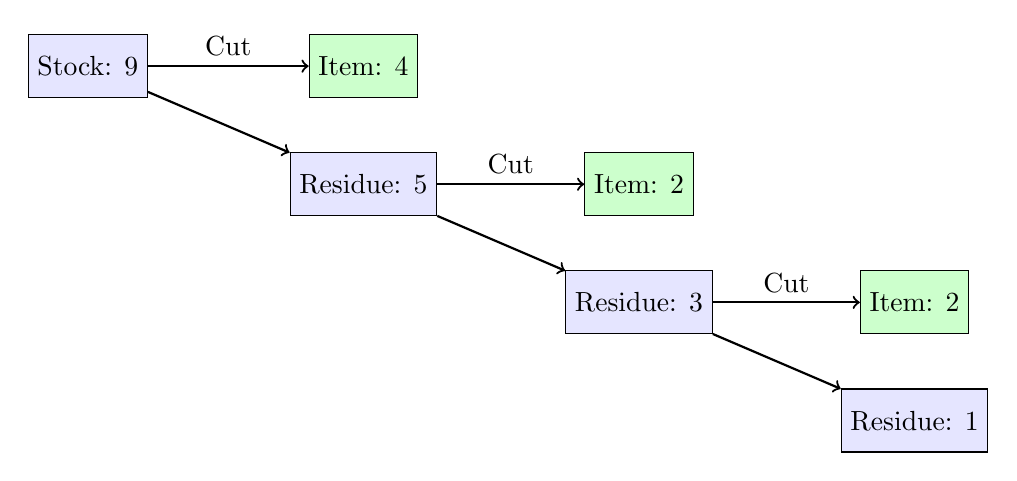
\begin{tikzpicture}[
        node distance=2cm,
        box/.style={draw, rectangle, minimum size=0.8cm, fill=blue!10},
        arrow/.style={->, thick}
    ]
        \node[box] (stock) {Stock: 9};
        \node[box, right of=stock, xshift=1.5cm, fill=green!20] (item1) {Item: 4};
        \node[box, below of=item1, yshift=0.5cm] (res1) {Residue: 5};
        
        \draw[arrow] (stock) -- node[above]{Cut} (item1);
        \draw[arrow] (stock) -- (res1);
        
        \node[box, right of=res1, xshift=1.5cm, fill=green!20] (item2) {Item: 2};
        \node[box, below of=item2, yshift=0.5cm] (res2) {Residue: 3};
        
        \draw[arrow] (res1) -- node[above]{Cut} (item2);
        \draw[arrow] (res1) -- (res2);
        
        \node[box, right of=res2, xshift=1.5cm, fill=green!20] (item3) {Item: 2};
        \node[box, below of=item3, yshift=0.5cm] (res3) {Residue: 1};
        
        \draw[arrow] (res2) -- node[above]{Cut} (item3);
        \draw[arrow] (res2) -- (res3);
    \end{tikzpicture}
    
    \vspace{0.2cm}
    \raggedright
    \small \textit{Each step produces one item and one smaller residual piece for further cutting.}
\end{frame}

\begin{frame}{Mathematical Formulation: Variables}
    Let $S$ be stock lengths, $D$ be demand lengths, and $R$ be valid residual lengths.
    
    \textbf{Decision Variables:}
    $$ y_{k,l} \ge 0 \quad \text{for } k \in S \cup R, \ l \in D, \ l < k $$
    
    \textbf{Interpretation:}
    \begin{itemize}
        \item $y_{k,l}$ represents the number of pieces of length $k$ that are cut to produce \textbf{one} item of order length $l$.
        \item This operation implicitly produces a residue of size $k-l$.
    \end{itemize}
\end{frame}

\begin{frame}{Mathematical Formulation: Constraints}
    The model relies on \textbf{Flow Conservation} for every length $l$ (Input $\ge$ Output).
    
    \begin{alertblock}{Flow Balance Constraint}
    For every length $l \in D \cup R$:
    $$ \underbrace{\sum_{k \in A_l} y_{k,l}}_{\text{Created by cuts}} + \underbrace{\sum_{k \in B_l} y_{k+l,k}}_{\text{Created as Residue}} \ge \underbrace{\sum_{k \in C_l} y_{l,k}}_{\text{Used for smaller cuts}} + \underbrace{N_l}_{\text{Final Demand}} $$
    \end{alertblock}

    \begin{itemize}
        \item \textbf{LHS:} Total availability of length $l$ (produced directly + leftover).
        \item \textbf{RHS:} Total consumption of length $l$ (cut into smaller items + shipped as demand).
    \end{itemize}
\end{frame}

\begin{frame}{Comparison: Model I vs. Model II}
    \begin{table}[]
        \centering
        \begin{tabular}{lll}
        \toprule
        \textbf{Feature} & \textbf{Model I (Gilmore-Gomory)} & \textbf{Model II (Dyckhoff)} \\
        \midrule
        \textbf{Variables} & Exponential (Patterns) & Polynomial (One-Cuts) \\
        \textbf{Constraints} & $|D|$ (Small) & $|D| + |R|$ (Larger) \\
        \textbf{Solver} & Column Generation & Standard Simplex \\
        \textbf{Structure} & Static Patterns & Dynamic Flow \\
        \bottomrule
        \end{tabular}
    \end{table}
    
    \textbf{Conclusion:} Model II is superior when the number of distinct lengths is moderate, as it avoids complex pricing subproblems.
\end{frame}

% -----------------------------------------------------------------------------
% METAHEURISTICS (GGA)
% -----------------------------------------------------------------------------

\section{Metaheuristics: GGA}

\begin{frame}{Why Metaheuristics? The Need for GGA}
    \textbf{Limitation of Classical Heuristics:}
    \begin{itemize}
        \item Greedy (FFD) gets stuck in local optima.
        \item Theoretical schemes (KK82) are computationally impractical ($N^{high}$).
    \end{itemize}
    
    \textbf{The Genetic Approach:}
    \begin{itemize}
        \item \textbf{Standard GA Failure:} Encoding solution as a list of items ($Item_i \to Bin_j$) creates a massive search space with redundancy (ordering doesn't matter).
        \item \textbf{The Solution (Falkenauer):} \textbf{Grouping Genetic Algorithm (GGA)}.
        \item \textbf{Core Idea:} The fundamental unit of evolution is the \textbf{Group (Bin)}, not the item.
        \item We evolve a population of \textit{packings}, preserving well-packed bins across generations.
    \end{itemize}
\end{frame}

\begin{frame}{The Cost Function: Navigating the Landscape}
    \textbf{Problem:}
    Minimizing the number of bins $N$ creates a ``flat'' fitness landscape. A solution with $N=10$ (mostly full) looks the same as $N=10$ (barely full). The algorithm has no gradient to follow.
    
    \textbf{Falkenauer's Objective Function:}
    Maximize the average ``fullness'' with non-linear scaling ($k>1$):
    $$ f_{BPP} = \frac{\sum_{i=1}^{N} (F_i / C)^k}{N} $$
    Where $F_i$ is the sum of items in bin $i$, $C$ is capacity, and $k=2$.
    
    \begin{block}{Why $k=2$?}
        It rewards ``extremist'' solutions. Two half-full bins score lower than one full bin + one empty bin. This drives the algorithm to completely fill bins and empty others.
    \end{block}
\end{frame}

\begin{frame}{The Crossover Operator (Group-Based)}
    Standard crossover destroys valid bin structures. GGA uses a specialized 4-step process:
    
    \begin{enumerate}
        \item \textbf{Selection:} Choose two parents. Select a set of ``best bins'' from Parent A to inject.
        \item \textbf{Injection:} Insert these bins into Parent B.
        \item \textbf{Elimination:} Some items now appear twice (once in the injected bins, once in Parent B's original bins). Remove the \textbf{original bins} in Parent B that contain these duplicates.
        \item \textbf{Re-insertion:} The items from the removed bins that were \textit{not} duplicates are now ``loose''. Re-insert them using a heuristic (FFD or Dominance).
    \end{enumerate}
    
    \textit{Result:} Offspring inherits high-quality compact bins from A, while adapting the rest.
\end{frame}

\begin{frame}{Mutation \& Local Optimization}
    \textbf{Mutation Strategy:}
    \begin{itemize}
        \item Randomly select a small number of bins.
        \item \textbf{Dissolve} them completely.
        \item Treat their items as ``loose'' and re-insert them.
        \item Purpose: Prevents premature convergence by forcing the algorithm to break up suboptimal local packings.
    \end{itemize}
    
    \textbf{The Role of Heuristics (Hybridization):}
    \begin{itemize}
        \item GGA relies heavily on a local heuristic for the ``Re-insertion'' phase.
        \item \textbf{Dominance Criterion (Martello \& Toth):} Prefer packings that dominate others (leave strictly less space or accommodate larger items).
        \item \textbf{Practical Implementation:} Often replaced by First-Fit Decreasing (FFD) or Best-Fit Decreasing (BFD) for speed during re-insertion.
    \end{itemize}
\end{frame}

% -----------------------------------------------------------------------------
% CONCLUSION
% -----------------------------------------------------------------------------

\section{Conclusion \& Hypothesis}

\begin{frame}{Summary of Algorithms Hierarchy}
    \begin{table}[]
    \begin{tabular}{lccc}
    \toprule
    \textbf{Algorithm} & \textbf{Type} & \textbf{Guarantee} & \textbf{Speed} \\ \midrule
    First-Fit & Online & $1.7 \cdot OPT$ & Fast \\
    Harmonic-$k$ & Online & $\approx 1.69 \cdot OPT$ & Fast \\
    FFD & Offline & $1.22 \cdot OPT$ & Fast \\
    Martello-Toth & Exact & Optimal & Exponential  \\
    Dyckhoff One-Cut & Exact LP & $(1+\epsilon)OPT + 1$ & Pseudo-Polynomial \\
    APTAS & Scheme & $(1+\epsilon)OPT + 1$ & Slow \\
    Karmarkar-Karp & Theoretical & $OPT + O(\log^2 OPT)$ & Very Slow \\
    Hoberg-Rothvoß & State-of-Art & $OPT + O(\log OPT)$ & Theoretical \\ \bottomrule
    \end{tabular}
    \end{table}
\end{frame}

\end{document}
